%for a more compact document, add the option openany to avoid
%starting all chapters on odd numbered pages
\documentclass[12pt]{cmuthesis}

% This is a template for a CMU thesis.  It is 18 pages without any content :-)
% The source for this is pulled from a variety of sources and people.
% Here's a partial list of people who may or may have not contributed:
%
%        bnoble   = Brian Noble
%        caruana  = Rich Caruana
%        colohan  = Chris Colohan
%        jab      = Justin Boyan
%        josullvn = Joseph O'Sullivan
%        jrs      = Jonathan Shewchuk
%        kosak    = Corey Kosak
%        mjz      = Matt Zekauskas (mattz@cs)
%        pdinda   = Peter Dinda
%        pfr      = Patrick Riley
%        dkoes = David Koes (me)

% My main contribution is putting everything into a single class files and small
% template since I prefer this to some complicated sprawling directory tree with
% makefiles.

% some useful packages
%\usepackage{times}
%\usepackage[defaultsans]{droidsans}
%\renewcommand*\familydefault{\sfdefault} %% Only if the base font of the document is to be typewriter style
%\usepackage[T1]{fontenc}

%\usepackage[sfdefault,light]{roboto}  %% Option 'sfdefault' only if the base font of the document is to be sans serif
\usepackage{libertine}
\usepackage[T1]{fontenc}

\usepackage{fullpage}
\usepackage{graphicx}
\usepackage{amsmath}
\usepackage[numbers,sort]{natbib}
\usepackage[backref,pageanchor=true,plainpages=false, pdfpagelabels, bookmarks,bookmarksnumbered,
%pdfborder=0 0 0,  %removes outlines around hyper links in online display
]{hyperref}
\usepackage{subfigure}
\usepackage{booktabs}

% Approximately 1" margins, more space on binding side
%\usepackage[letterpaper,twoside,vscale=.8,hscale=.75,nomarginpar]{geometry}
%for general printing (not binding)
\usepackage[letterpaper,twoside,vscale=.8,hscale=.75,nomarginpar,hmarginratio=1:1]{geometry}

% Provides a draft mark at the top of the document.
\draftstamp{\today}{DRAFT}

\begin {document}
\frontmatter

%initialize page style, so contents come out right (see bot) -mjz
\pagestyle{empty}

\title{ %% {\it \huge Thesis Proposal}\\
{\bf Visualization and Management of Large Structured Biological Data}}
\author{Darya Filippova}
\date{July 2015}
\Year{2015}
\trnumber{}

\committee{
Carl Kingsford, Chair \\
Takis Benos \\
Russel Schwartz \\
Liz Marai, U of Illinois
}

\support{This research was supported in part by \ldots}
\disclaimer{}

% copyright notice generated automatically from Year and author.
% permission added if \permission{} given.

\keywords{Stuff, More Stuff}

\maketitle

% TODO: enable dedication
%\begin{dedication}
%For my dog Coco and her uncle Shiloh
%\end{dedication}

\pagestyle{plain} % for toc, was empty

%% Obviously, it's probably a good idea to break the various sections of your thesis
%% into different files and input them into this file...

\begin{abstract}
% A short summary -- one page.

% The problem.
Advances in biological technology over the last decade allow us to capture biologically meaningful data on a scale not possible before. Carefully designed experimental protocols now allow scientists to capture protein-protein interactions, dependencies between genes, their products, and metabolites for tens of thousands of targets at a time. At the same time, rapid evolution of sequencing technologies made whole genome and accurate transcriptome analyses possible. However, large amounts of data generated in these high-throughput biological experiments make data storage, analysis, and visualization difficult.
% Significant advances and contribute to our understanding and knowledge.
This dissertation discusses several analysis and visualization challenges in detail, and presents efficient and flexible solutions. %advancing our understanding of the underlying data and adding to existing body of knowledge.
First part of the dissertation identifies problems of presenting large structured data  and discusses the interfaces and processes designed to address them.
% Designed interfaces and explored their usability.
Designed algorithms and analysis techniques.

Conclusions and contributions that came out of this work.

\end{abstract}

\begin{acknowledgments}
CK. Ben Shneiderman. Rob Patro and Geet Duggal. All members of CK lab.

Michael Pack.

My collaborators.

People who taught me resilience.

My family for support, especially my mom.
\end{acknowledgments}



\tableofcontents
\listoffigures
\listoftables

\mainmatter

%% Double space document for easy review:
%\renewcommand{\baselinestretch}{1.66}\normalsize

% The other requirements Catherine has:
%
%  - avoid large margins.  She wants the thesis to use fewer pages,
%    especially if it requires colour printing.
%
%  - The thesis should be formatted for double-sided printing.  This
%    means that all chapters, acknowledgements, table of contents, etc.
%    should start on odd numbered (right facing) pages.
%
%  - You need to use the department standard tech report title page.  I
%    have tried to ensure that the title page here conforms to this
%    standard.
%
%  - Use a nice serif font, such as Times Roman.  Sans serif looks bad.
%
% Other than that, just make it look good...


\chapter{Introduction}

\section{Background}

\section{Aims/Challenges}

Also -- challenges

\section{Major contributions}

%%%%%%%%%%%%%%%%%%%%%%%%%%%%%%%%%%%%%%%%%%%%%%%%%%%%%%%%%%%%%%%%%%%%%%%%%%%%%%%%
%%%%%%%%%%%%%%%%%%%%%%%%%%%%%%%%%%%%%%%%%%%%%%%%%%%%%%%%%%%%%%%%%%%%%%%%%%%%%%%%
%%
%%
%%
%% Part 1 -- visualizaiton for biological data
%%
%%
%%
%%%%%%%%%%%%%%%%%%%%%%%%%%%%%%%%%%%%%%%%%%%%%%%%%%%%%%%%%%%%%%%%%%%%%%%%%%%%%%%%
%%%%%%%%%%%%%%%%%%%%%%%%%%%%%%%%%%%%%%%%%%%%%%%%%%%%%%%%%%%%%%%%%%%%%%%%%%%%%%%%
\part{Visualization approaches for large structured data}


%%%%%%%%%%%%%%%%%%%%%%%%%%%%%%%%%%%%%%%%%%%%%%%%%%%%%%%%%%%%%%%%%%%%%%%%%%%%%%%%
%%
%% Map of jazz -- dynamic network vis
%%
%%%%%%%%%%%%%%%%%%%%%%%%%%%%%%%%%%%%%%%%%%%%%%%%%%%%%%%%%%%%%%%%%%%%%%%%%%%%%%%%
\chapter{Visualizing dynamic networks with context}
% map of jazz

Intro to chapter -- why visualization is important (quartet dataset), visualizing 1000 data points in one pixel, formulating hypotheses that may not be obvious from computing standar statistical measures.

Which visualization problems we tackle.

Research presented in this chapter is partially represented in publications~\cite{Filippova2012moj},
~\cite{Coral}, and~\cite{SHARQwebsite}.

\section{Background}

  XXX

  (abstract from the paper)

  We present a new system for exploring, in an intuitive and interactive way, a
  large compendium of data about collaborations between jazz musicians.  The
  system consists of an easy-to-use web application that marries an ego-network
  view of collaborations with an interactive timeline.  We develop a new measure
  of collaboration strength that is used to highlight strong and weak
  collaborations in the network view. The ego-network is arranged using a novel
  algorithm for ordering nodes that avoids occlusion even when the network is
  frequently changing. Finally, the system is applied to a large, unique,
  hand-curated data set of recorded jazz collaborations.
  The system can be accessed at \url{http://mapofjazz.com/socialcom}.

  (intro from the paper)

  The evolving community of jazz musicians is an example of a social network where
  personal connections are essential~\cite{Pinheiro2009}. In jazz, a highly
  collaborative art form, one person's individual style is shaped by constant
  experimentation and exchange of techniques and ideas with fellow
  musicians~\cite{Berliner1994}.  Every musician is part of a dense network of
  collaborators with many transient connections: a composer may arrange music for
  multiple bands simultaneously, band leaders may recruit new members to their
  bands and lose them to competition, or musicians' skills may improve to the
  point where they are featured as soloists and have a prominent place in the
  band. Study of recorded jazz collaborations can help identify influences on
  style, explain career success, and lead to a richer understanding of the
  progression of the jazz art form.

  The traditional means by which these collaborations are explored is via the
  compilation and study of discographies presented as lists and tables in either
  hard-copy books or in computerized databases~\cite{Timner2007,Albin}. These
  discographies list recording sessions, the roles each musician played in them,
  often songs and albums that were produced as a result, along with other
  information. They provide an extremely rich source of information from which to
  trace the collaborations of musicians. However, such a static and textual
  presentation is difficult to comb through and does not easily allow the user
  to comprehend the dynamics of changing collaborations.
  While changes in band membership are easily traceable, it is hard to assess the
  overall contribution of a band member over time unless the historians are
  intimately familiar with the band's history.
  A system for exploring
  jazz collaborations that makes large discography data more approachable
  is needed.

  Social networks such as those between collaborators or friends are an object of
  intense study. Often, such connections are assumed to be immutable and the
  networks are considered static. However, there are many social interactions
  that violate this assumption: work colleagues, neighbors, acquaintances,
  friends, and family may all change over the course of a person's lifetime. This
  is particularly true of jazz collaborations where band members frequently come
  together for only a single recording session, and where some musicians have
  played with over a thousand other artists over their decades-long careers.
  Understanding changes in connectivity on a scale of the whole network can provide
  an insight about the global change within the network, but has proven to be a
  difficult task for both algorithmic~\cite{Hopcroft2004, Palla2005c,
  Tantipathananandh2007, TangLiuZhna08} and visualization~\cite{BenderDeMoll2006,
  Rosvall2010,Yi2010} approaches.  The dynamism of jazz collaborations requires
  new approaches to visualize frequently changing networks.

  Apart from the topological changes, there may be other, more subtle variations
  in the characteristics of relationships over time.  Node or edge attributes may
  change, e.g.\@ the relationship between $A$ and $B$ may gradually change from
  an acquaintance to a close collaboration, or the ``importance'' of $A$'s
  immediate collaborators may grow, thus indirectly increasing the importance of
  $A$ itself.  Collectively, such changes may affect the profile of an individual
  in a significant way, but these observations are lost in the sea of data when
  analyzing the network as a whole. This, along with a traditional focus on the
  lives of individual musicians, leads to the desire to have a visualization that
  can be focused on subregions of the entire space of collaborations. It also
  leads to the need for techniques to quantify the strength of the relationships
  encoded in an evolving network and to show this information effectively through
  a visualization.


  \subsection{Dynamic network visualization}

  There are two main approaches to visualizing time-varying networks: to show
  animations by constantly recomputing layouts at every time step~\cite{Yee2001}
  and to compare
  static snapshots of a network at several distinct time points. For either
  approach, the objective is to highlight the differences between the network
  views at different time steps.

  Brandes and Corman~\cite{Brandes2003a} stack network snapshots on top of each
  other in 3D where the nodes with the same labels are connected by vertical columns.
  The graph is laid out using a spring-embedded algorithm, and each slice shows
  only the nodes and edges present at that time point. Yim, Shaw, and
  Bartram~\cite{Yim2009} show a snapshot of a network in its early state and
  indicate changes in node positions with red arrows leading to complicated and
  cluttered displays. Diehl and G\"{o}rg~\cite{Diehl2002} place the two network
  snapshots side by side and propose three algorithms that minimize
  dissimilarities between the two representations. A recent study by Khurana et
  al.~\cite{Khurana2011} presents an extension to NodeXL~\cite{Bonsignore2009}
  that aggregates the snapshots of a network at two different time points into a
  single view. The edges are colored based on the time interval at which they
  existed. Additionally, NodeXL plots the values of several common graph
  properties such as node and edge counts as they change over time between the two
  time points. An approach by Yi et al.~\cite{Yi2010} combines a small multiples
  display (a histogram showing node degree over time) and a matrix representation
  of a network into a single view.

  Graph layout for the animations may be fixed or constantly updating at each time
  step. Moody et al.~\cite{Moody2005} keep the node positions fixed and allow the
  edges to appear and disappear as the time progresses in their \emph{flip-book}
  animations. Yee and colleagues~\cite{Yee2001} allow the nodes to move between
  the concentric circles along a smooth tangential trajectory.

  While these approaches are able to highlight the topological changes, they all
  make an assumption that node and edge attributes (such as edge length) are
  either absent or remain static over time.

  % related work: circular layouts

  \subsection{Circular and ego-network layouts}

  As early as 1990, circular layouts were used for organizing trees by placing the
  root in the center and assigning the child nodes to concentric circles with
  increasing radii~\cite{North1997}, with nodes at the same level of a tree
  assigned to the same circle. Six et al.~\cite{Six1999}
  extended the technique to work for more general graphs by connecting multiple
  circular structures. Yee and colleagues~\cite{Yee2001} have developed the technique
  further to support nodes of different sizes (where node size is proportional
  to some node attribute). They adapted their layout to handle dynamic graphs by
  showing animations of nodes traveling on a smooth trajectory from old
  locations to the new ones.

  Wang, Shi, and Wen~\cite{Wang2011a} experiment with a dynamic ego-network design
  where the central node and all of its connections are shown at the same time.
  The main node has several copies with each one representing the node at a
  specific point in time and linked only to those nodes with which it was
  associated during that period. This approach is not feasible if the
  central node has many collaborators over his or her career.

  Gansner and Koren~\cite{Gansner2006} develop
  heuristics that order nodes on a circle's periphery in a way that minimizes the
  edge crossovers and reroutes some of the links to go outside the circle's
  circumference. These authors suggest edge bundling for the links inside the circle to
  reduce clutter further. Their work does not consider dynamically changing links.

  % related work: collaboration networks

  \subsection{Artist collaboration networks}

  Artist collaboration networks have received their fair share of attention in
  social network analysis. The data on interactions among misicians is available
  in some databases~\cite{Gleiser2003,Pattuelli2012}, has been collected through
  surveys~\cite{Heckathorn2001a}, or assembled manually by processing the tapes of
  interviews with the artists~\cite{Pattuelli2011}. Due to difficulties in data
  collection, these sources cover only a few artists and lack
  temporal information about their collaborations. For example, Gleiser and
  colleagues~\cite{Gleiser2003} base their analysis on 198 bands that were active
  in 1912-1940. Heckathorn and Jeffri's survey reached out to 110 musicians in
  New Orleans, 264 in New York, and 300 in San Franscisco~\cite{Heckathorn2001a},
  a small fraction of the estimated 33,000 jazz musicians living in New York.

  Examples of applications supporting exploration of such networks are few. An
  online Classical Music Navigator~\cite{Smith1999} helps users expand their
  musical interests by suggesting composers who influenced or were influenced by
  a composer the users initially searched for. The Navigator offers a simple text
  and link interface. A visualization of Last.fm data~\cite{Bieh-Zimmert2011}
  allows one to compare two artists and their musical associations, but does not
  provide any intuition about collaborations between the two artists.

  In this paper, we propose a way to quantify the strength of collaboration
  between two actors in the network based on the frequency and timing of the
  events in which they have both participated. We provide a visualization system
  that displays much of the data available in large discographies. In this
  network, nodes represent artists and edges connect artists who participated in
  the same recording session at some time. We visualize creative partnerships
  between musicians using an interactive egocentric network
  view that allows users to focus on an individual and observe large and small
  scale changes in collaborations (Fig.~\ref{fig:map}). We couple this network
  view with an interactive
  timeline that allows the user to see how the strength of ties changed over time.
  We also introduce a novel algorithm that arranges collaborator nodes around the
  central musician in a way that minimizes node occlusion and variation in node
  positions as the network view changes over time. This helps the users to
  maintain their mental map of evolving collaborations. We demonstrate the utility
  of this approach on an extensive hand-curated collection of jazz collaborations
  spanning almost a hundred years.

\section{Dynamic network data}

  % Describe the process of entering, cleaning, improving, expanding,
  % cross-referencing.

  The Map of Jazz uses data that have been collected over the course of more than
  twenty years of discographical research, with additional content subsequently
  added in targeted batches. The data come from a myriad of sources: from general and
  artist discographies to specialist journals, magazines, and newsletters to
  biographical and historical monographic literature and many more. In almost
  every case, a single entry is a collection of data from multiple sources because
  no one source covers every aspect of the recording session. The sessions cover a
  period of time from the early 1920s to the present day.

  While there have been other attempts at digitizing discographical information,
  these used closed, proprietary systems that lacked both the ability to export
  and import or edit the information, and ultimately were unable to satisfy the
  information needs of serious researchers. The data used by the Map of Jazz were
  collected and stored using the open-source discographical software
  BRIAN~\cite{Albin}, named so for the English discographer Brian Rust who
  perfected the session-based format for print
  discographies~\cite{Rust1980,Rust2002}.
  BRIAN's support for data export and import allowed for
  multiple users to contribute to the project and amounted to a large number of
  cataloged recording sessions. The Map of Jazz is the first project to use large
  amounts of BRIAN data outside of the application itself.

  At the heart of BRIAN is the conceptual idea that the session is the
  primary entity, unlike many other databases designed to store sound recordings
  information. Sessions are events that have defined locations, both
  chronologically and geographically. Out of the many layers of details available
  in BRIAN, the Map of Jazz uses the top-level data on the sessions and musicians
  who performed during them, thus shifting the focus to the interpersonal
  relationships between the artists. The attribute for the main musical instrument
  helps to distinguish Bill Evans the saxophonist from Bill Evans the pianist; it
  also records what instrument each performer played.
  %
  % Top 5 guys by the number of collaborators
  %
  \begin{table}
    \centering
    \begin{tabular}{l  r}
    \toprule
    Name & Degree \\
    \midrule
    Slide Hampton & 1230\\
    Kenny Barron & 1090\\
    Ron Carter & 785\\
    Michael P. Mossman & 692\\
    Freddie Hubbard & 691\\
    \bottomrule
    \end{tabular}
    \caption{Top 5 musicians with the highest number of collaborations. Slide
    Hampton was a prolific composer who has provided arrangements for multiple
    bands, hence his interaction surpasses that of many famous band leaders.}
    \label{tab:high_degree}
  \end{table}
  %

  % Data statistics.

  At the time of publication, the database contained information on 11824
  musicians and a total of 13873 recording sessions. The average number of people
  per recording session was 7.39 with the smallest sessions having just one
  performer, and the largest session having 72 people (not including the members of
  symphony orchestras). Network diameter (the longest among all shortest paths between all
  pairs of vertices) was equal to 8, and the average (\emph{characteristic})
  shortest path was equal to 3.24. As with many social networks, very few
  musicians have a high number of connections, with an overall average node degree
  of 33.68 (see Fig.~\ref{tab:high_degree} for the top 5 artists by degree).
  However, the network does not pass the test for scale-freeness according to the
  test developed by Clauset et al.~\cite{Clauset2009b} suggesting that the network
  has evolved by processes other than the well-studied ``rich get richer"
  mechanism.

%%%%%%%%%%%%%%%%%%%%%%%%%%%%%%%%%%%%%%%%%%%%%%%%%%%%%%%%%%%%%%%%%%%%%%%%%%%%%%%%
%\section{Results and discussion}

\section{Interface design}
  The Map of Jazz focuses on the dynamics within the collaboration networks of
  individual musicians.
  An egocentric network layout (Fig.~\ref{fig:map})
  is coupled with an interactive timeline that allows
  users to navigate through various time periods and observe gradual changes in
  the person's collaboration network.
  The timeline is augmented with aggregate statistics, such as the number of
  people per sessions, to aid in navigation through time.
  In the network view,
  nodes representing collaborators are arranged around the central node in a
  manner that preserves nodes' relative positions across time and shows the
  relative strength of a tie between the main musician and his or her collaborator.
  Nodes and edges used in the traditional node-link network representation are
  extended to display the change in attribute values over time.
  Finally, the interactions between the currently displayed main musician's
  collaborators can be explored on demand by highlighting a node of interest which
  reveals its connections to other nodes in the neighborhood. The central
  artist can be selected by double-clicking on
  a performer's node or by entering a musician's name in a search box. To help
  users pick a starting point, the Map of Jazz offers a dropdown with 21
  hand-picked sessions that stand out in jazz history.

  %%%%%%%%%%%%%%%%%%%%%%%%%%%%%%%%%%%%%%%%%%%%%%%%%%%%%%%%%%%%%%%%%%%%%%%%%%%%%%%%
  %
  % Visual: timeline
  %
  %%%%%%%%%%%%%%%%%%%%%%%%%%%%%%%%%%%%%%%%%%%%%%%%%%%%%%%%%%%%%%%%%%%%%%%%%%%%%%%%

  \subsection{Timeline}

  Users may navigate the extensive Map of Jazz timeline by dragging it with a
  mouse. They may also zoom in on a particular period of the musician's life or
  zoom out to get an overview of the artist's career. Every time the users
  interact with the timeline, the ego-network is updated to present an accurate
  snapshot for the selected time period.

  \textbf{Sessions.} The triangles on the timeline represent recording sessions
  (Fig.~\ref{fig:timeline}). When users hover
  over the triangle with a mouse, the session and the collaborators who recorded for
  that session are highlighted in yellow. Users may click on a session to select
  all the participating collaborators and the session itself, and vice versa. A
  tooltip that appears above the triangle icon
  summarizes the information about the session: the date, location, and
  a list of participating musicians along with their primary skill (an instrument
  they played, e.g.~alto saxophone, or a role they took, e.g.~band leader, during
  a session).

  When the date of birth and/or death are available, the span of time from birth
  to death (or to the present day) is colored in a lighter shade of gray to
  indicate the span of the musician's life.
  %
  \begin{figure}
    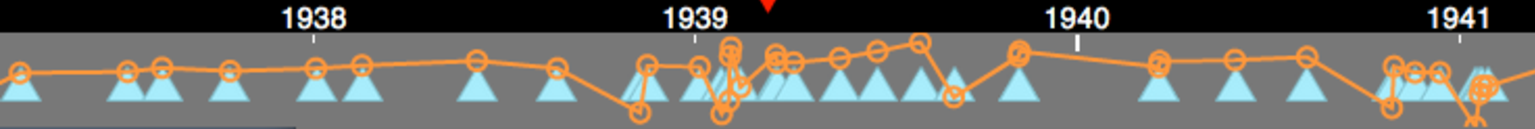
\includegraphics[width=\linewidth]{timeline}
    \caption{A timeline augmented with a session similarity graph. Triangles
  represent the individual recording sessions. Most sessions on the
  timeline have a high pairwise similarity indicating that session memberships
  changed only slightly.}
    \label{fig:timeline}
  \end{figure}
  %
  \textbf{Augmented timeline.} To aid users in focusing on a specific time period
  of interest, the Map of Jazz offers several basic metrics to be overlaid on top
  of the timeline. These include:
  %
  \begin{itemize}
    \item the number of collaborators per session,
    \item the number of unique musicians the person collaborated with up to this date,
    \item the Jaccard similarity between the members of the current session and
    the previous session.
  \end{itemize}
  %
  The number of collaborators and the speed at which a person attracts new
  collaborators have been shown to be significant in scientific~\cite{Petersen2012}
  and jazz~\cite{Pinheiro2009} collaborations, while the session size may explain
  the mechanism of acquiring new collaborators (i.e. switching between bands
  versus playing with the same band).


  %%%%%%%%%%%%%%%%%%%%%%%%%%%%%%%%%%%%%%%%%%%%%%%%%%%%%%%%%%%%%%%%%%%%%%%%%%%%%%%%
  %
  % Implementation: influence function
  %
  %%%%%%%%%%%%%%%%%%%%%%%%%%%%%%%%%%%%%%%%%%%%%%%%%%%%%%%%%%%%%%%%%%%%%%%%%%%%%%%%

  \subsection{Measure of collaboration strength}

  The notion of mutual influence between any two musicians lies at the heart of
  the Map of Jazz.
  To quantify the strength of the relationship between any pair of musicians, we
  make an assumption that the recording sessions are not spontaneous events,
  but rather a result of previous undocumented collaboration (e.g. concerts and
  rehearsals). Consequently, the professional relationship between the musicians
  is not likely to start right before a session nor to stop immediately after
  recording it, but rather to grow before the session and wane gradually over
  time. The collaboration is strongest around the
  time of a recording session and is increased even more if the musicians record
  several sessions over a short period of time.
  With these assumptions in mind, we define a function of
  \emph{collaboration strength} that takes into account the frequency and
  proximity in time of the collaborations between the two musicians:
  %
  \begin{equation}\label{eqn:influence}
  %
  g(t; S, \sigma) = \alpha_\sigma \sum_{s \in S} e^{-\beta_\sigma(t_s-t)^2 },
  %
  \end{equation}
  %
  where $S$ is the set of all sessions the two musicians shared, $t$ is a point in
  time for which we want to evaluate the collaboration strength (i.e.\@ the center
  of the timeline), and $t_s$ is the date for a specific session $s$. To make the
  decay of the collaboration strength smooth, we model it as a normal distribution
  with $\alpha_\sigma = 4/(\sigma^2\sqrt{2\pi})$ and $\beta_\sigma = 1/(2\sigma^2)$.
  %
  The function~\eqref{eqn:influence} is similar to a kernel density estimator for
  normally distributed values, where choosing the bandwidth for the kernel is a
  known hard problem. To make the function smooth, we take an affine combination
  of two functions:
  %
  \begin{equation}\label{eqn:influence2}
  %
  f(t; S) = \delta g(t; S, \sigma_1) + (1-\delta)g(t; S, \sigma_2),
  %
  \end{equation}
  %
  with $\sigma_1 = 1$, $\sigma_2 = 3$, and $\delta=0.9$. The resulting function
  assigns more impact to the interactions that were closer to $t$ in time rather
  than assign an equal weight to all interactions no matter how long ago, or how
  far in the future, they occurred (Fig.~\ref{fig:infl_func}).

  %TODO: Unlike the function used in~\cite{Palla2005c}), we take into account both
  %the past and the future collaboration events.

  \begin{figure}
   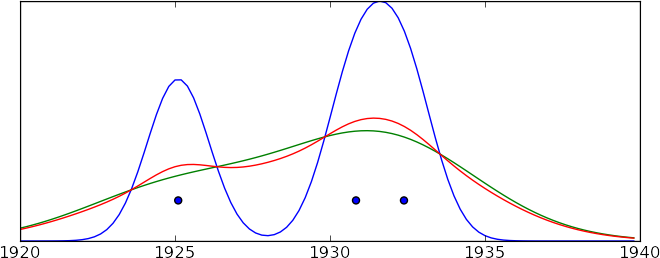
\includegraphics[width=\linewidth]{influence_plot.png}
   \caption{The collaboration strength function (red) is a combination of two functions:
    one for which  the value grows fast as $t$ gets closer to the session (blue)
    and another one for which the change in value is much smoother (green).
    Here, two hypothetical
    musicians played together in 1925, 1930, and 1932 (blue dots). Their
    relationship is strongest when several sessions occur within a short period of
    time such as in 1930--1932. The collaboration strength drops slightly between
    1925 and 1930 and declines rapidly after the last session in 1932.}
   \label{fig:infl_func}
  \end{figure}


  %%%%%%%%%%%%%%%%%%%%%%%%%%%%%%%%%%%%%%%%%%%%%%%%%%%%%%%%%%%%%%%%%%%%%%%%%%%%%%%%
  %
  % Visual design: egonetwork
  %
  %%%%%%%%%%%%%%%%%%%%%%%%%%%%%%%%%%%%%%%%%%%%%%%%%%%%%%%%%%%%%%%%%%%%%%%%%%%%%%%%
  \subsection{Egocentric network view}

  An egocentric view allows the user to track the fluctuating interactions between
  a given musician and his or her peers over time. Using the timeline, users may
  select a time range of interest and focus on the collaborations between the main
  musician and his or her collaborators within that period. Only the collaborators
  that were involved in sessions that occurred during that time range will be
  shown. For every collaborator $v$, we compute the collaboration strength between
  the center musician $u$ and $v$ where $S$, the set of sessions considered in the
  collaboration strength function, equals the sessions that are currently visible on
  the timeline. The length of an edge connecting $u$ and $v$ is inversely
  proportional to the strength of the tie shared by the two artists, as measured
  by the collaboration strength function~\eqref{eqn:influence}. This causes the
  collaborators who record with the main musician $u$ often or have recorded with
  him or her recently to be placed closer to the center, while musicians who
  record with $u$ rarely or have only recorded with $u$ a long time ago are placed
  on the periphery (Fig.~\ref{fig:map}).

  As users drag the timeline, the collaborators' nodes may move closer to the
  center or may drift away to the periphery as the set of sessions that is
  displayed changes. Nodes disappear from view when they are no longer involved in
  any session that is visible on the timeline, and new nodes appear when sessions
  containing them come into view on the timeline. To minimize the cognitive load
  on the users, the Map of Jazz preserves the angular positions for every
  collaborator node within the ego-network formed by a particular main musician.
  For every musician $u$, we assign a unique angular sector to every collaborator
  $v$ who has ever recorded with $u$ (Fig.~\ref{fig:ordering}). Their trajectory,
  a straight line connected to the center, can be easily traced as collaborator
  nodes move to or from the center.

  If care is not taken with the assignments of nodes to angular sectors, collaborators may
  crowd near the center if the main musician consistently played with the same
  set of people (i.e.\@ their band). To avoid this, we propose an ordering
  algorithm in Section~\ref{sec:ordering} to arrange the collaborator nodes in a
  way that assigns dissimilar angles to collaborators with which the center node
  has had similar patterns of collaboration.

  %TODO: highlight nodes that just showed up OR have a session with the main guy
  %withing $\epsilon$ distance of $t_{center}$

  %[XXX (move to ego-net) Users control the animation between two different states
  %by zooming in and out of the timeline and by dragging the timeline left or
  %right. These actions change the $t_c$ time thus causing layout to update.]

  %%%%%%%%%%%%%%%%%%%%%%%%%%%%%%%%%%%%%%%%%%%%%%%%%%%%%%%%%%%%%%%%%%%%%%%%%%%%%%%%
  %
  % Implementation: ordering collaborators
  %
  %%%%%%%%%%%%%%%%%%%%%%%%%%%%%%%%%%%%%%%%%%%%%%%%%%%%%%%%%%%%%%%%%%%%%%%%%%%%%%%%

  \subsection{Ordering collaborators in a circle}
  \label{sec:ordering}

  % TODO: Test how heterogeneous/homogeneous interaction are over time for most
  %people? High degree ppl? Low degree ppl?

  The Map of Jazz maintains the same angular node positions across every time
  period, allowing easier comparison of the network at different time points. As
  users navigate the timeline, new nodes may show up on the map, but they will
  never change the angular position of the nodes already on screen, thus
  preserving the users' mental map of the ego-network.

  The permanent angular node positions also help alleviate another problem common
  to graph drawing: node occlusion. More often than not, jazz musicians have a
  band, or several bands, with which they play and record on a regular basis. In
  this case, every person in the band would share a strong tie with the musician
  in question. The Map's circular layout would try to place all such frequent
  collaborators near the center, causing the nodes and labels to occlude each
  other.

  To minimize such occlusions, we identify groups of people that are likely to be
  at the same distance from the central node at the same time. To find the groups,
  we first sample the collaboration strength function values between the main
  musician $u$ and each one of its collaborators $v$:
  %
  \begin{equation}\label{eqn:sample}
  %
    x_{u, v} = (f(t_1;S), f(t_2;S), \ldots, f(t_{1000};S)),
  %
  \end{equation}
  %
  where $t_i$ are equally spaced time points in the range
  $[t_\textrm{min}, t_\textrm{max}]$ with $t_\textrm{min}$ equal to the date of
  $u$'s earliest session and $t_\textrm{max}$ equal to the date of $u$'s last
  recording session. In~\eqref{eqn:sample}, $S$ is the set of all the sessions in
  which the central node $u$ participated.
  %
  Next, we construct a pairwise similarity matrix for all $u$'s,
  $M_u = \left(m^u_{i,j}\right)$,
  where $m^u_{i, j}$ is the cosine similarity between vectors $x_{u,v_i}$ and
  $x_{u,v_j}$. To make it easier for the clustering algorithm to find groups in
  this matrix, we set every $m^u_{i,j} < 0.9$ to $0$. The resulting sparse matrix
  $M'_u$ is taken as a weighted adjacency matrix of a graph $G_u$. We run the
  Louvaine clustering algorithm~\cite{Blondel2008}, which attempts to find
  clusters maximizing modularity~\cite{newman06}, on $G_u$ to identify groups
  of musicians for whom the $x_{u, v_i}$ vectors were similar.

  Performers in the same cluster interact with the main performer in a similar
  fashion. To spread them out, we assign them sectors of the circle that are far
  from each other.
  %
  \begin{figure}[ht]
    \centering
    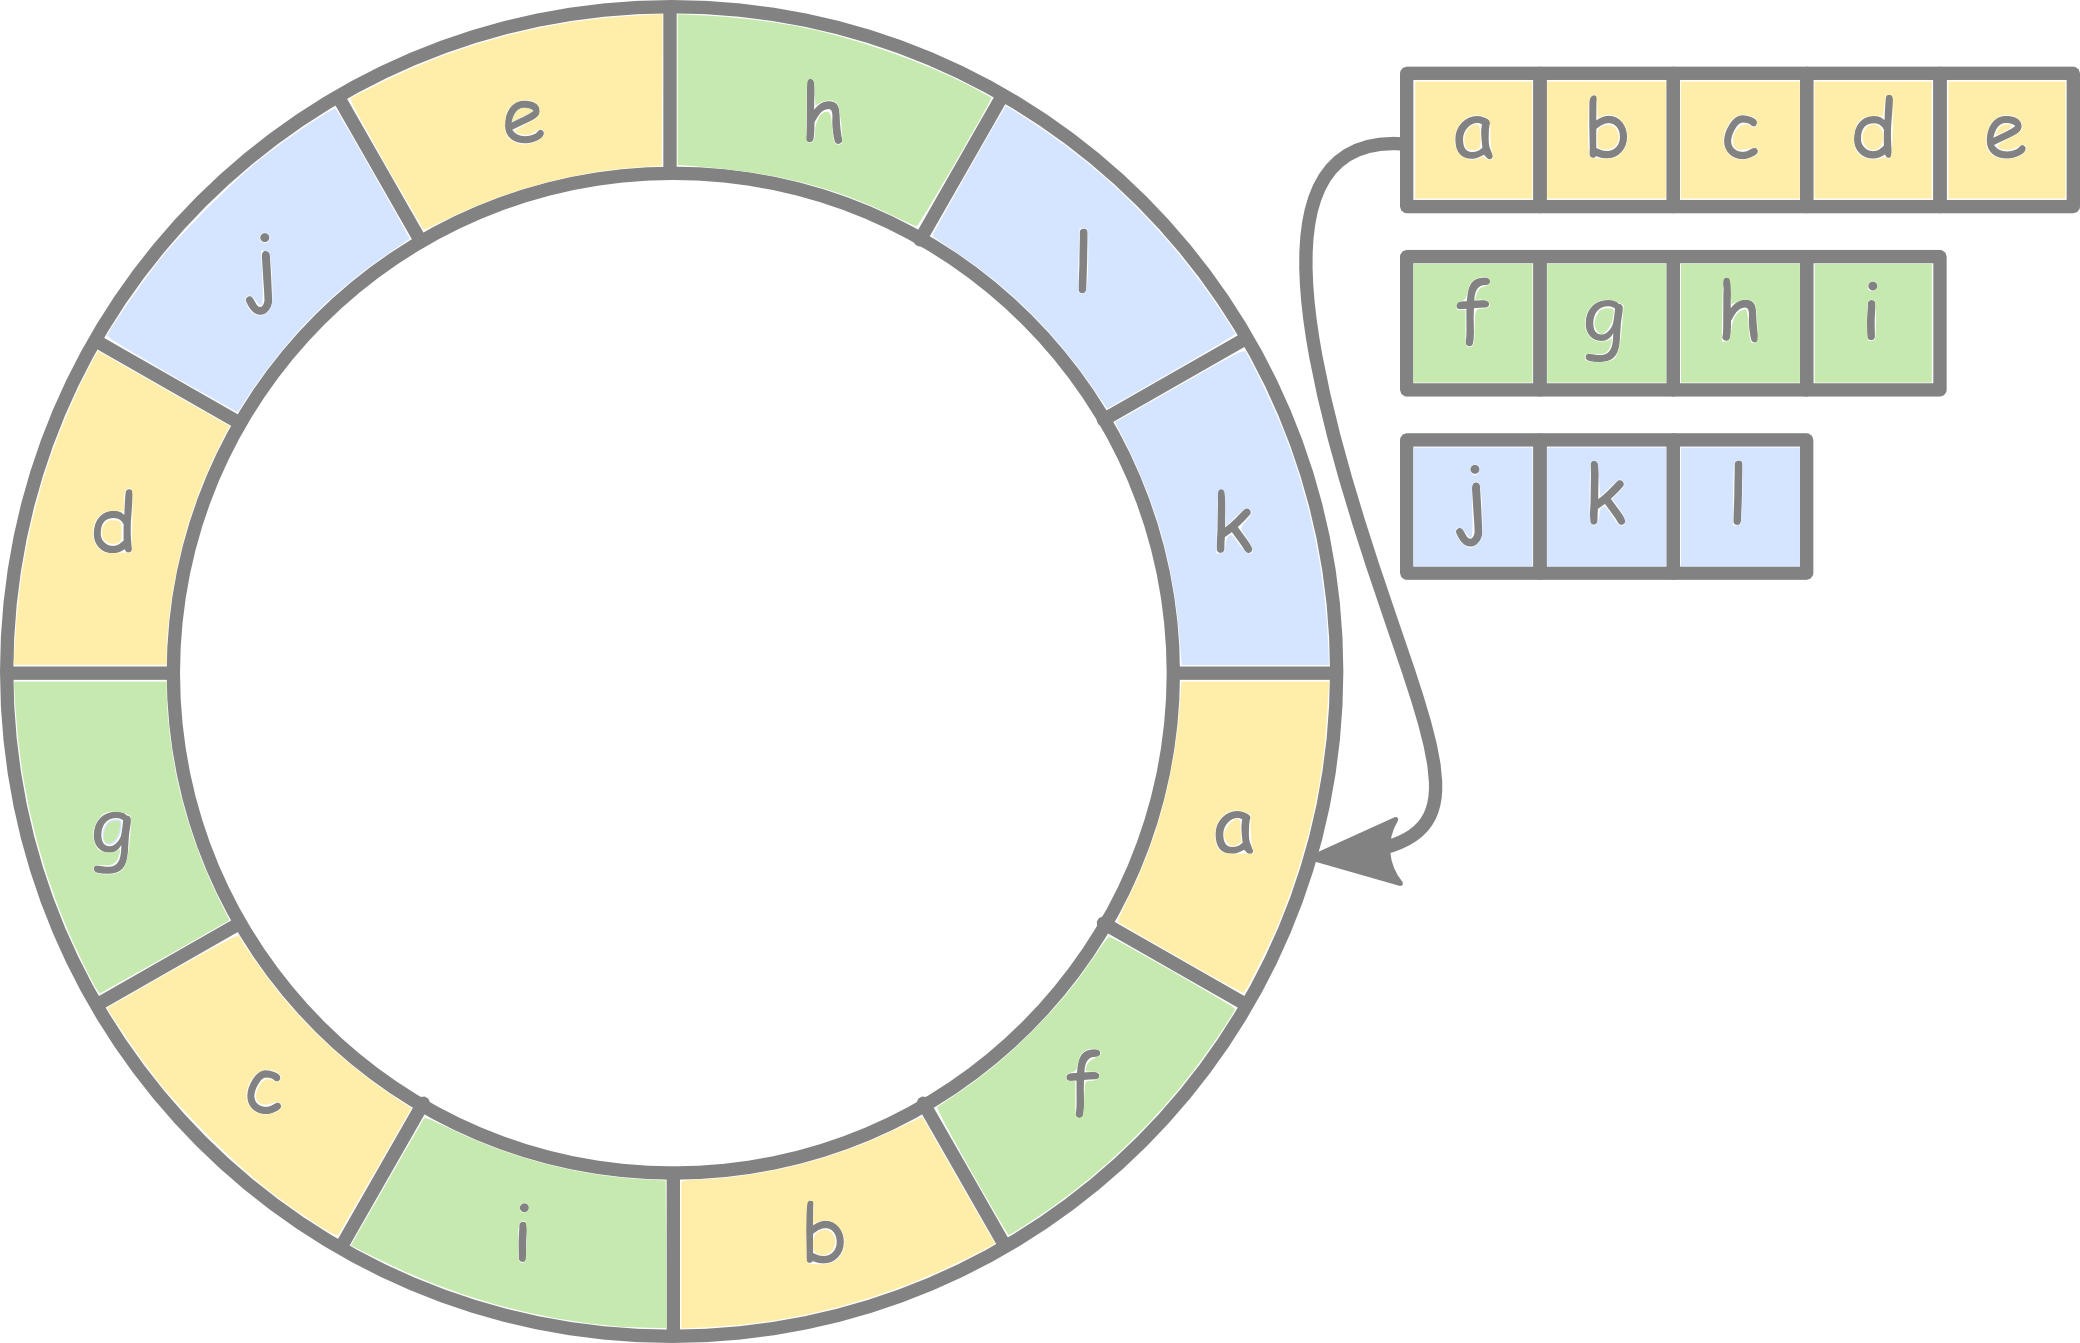
\includegraphics[width=\linewidth]{ordering}
    \caption{Assigning angular positions for the nodes. Starting with the largest
    cluster, performers from the same cluster get assigned sectors of the circle
    that are far from each other. Here, \emph{a} is assigned to the $1^\textrm{st}$
    sector, \emph{b} is $\left\lfloor \frac{12}{5} \right\rfloor = 2$ sectors away, and so on.}
    \label{fig:ordering}
  \end{figure}
  %
  To assign all $N$ collaborators to their angular positions, we iterate through
  the clusters in order of decreasing size.  For each cluster $C$, we assign a
  node in $C$ to the first empty sector and continue assigning $v \in C$ to empty
  sectors evenly around the circle at intervals of
  $\left\lfloor\frac{N}{|C|}\right\rfloor$
  sectors.  If at any time the target sector is not empty, we search linearly
  clockwise for the next available sector and continue assigning the remaining
  nodes in $C$ starting from that sector (Fig.~\ref{fig:ordering}). This
  heuristic --- similar to linear reprobing in a hash table --- attempts to
  ensure that the nodes belonging to the same cluster are spread out around the
  circle at equal intervals.

  %%%%%%%%%%%%%%%%%%%%%%%%%%%%%%%%%%%%%%%%%%%%%%%%%%%%%%%%%%%%%%%%%%%%%%%%%%%%%%%%
  %
  % Visual: Node glyphs
  %
  %%%%%%%%%%%%%%%%%%%%%%%%%%%%%%%%%%%%%%%%%%%%%%%%%%%%%%%%%%%%%%%%%%%%%%%%%%%%%%%%

  \subsection{Node and edge glyphs}

  A static snapshot of a collaboration ego-network may be misleading due to the fact
  that the past and future collaborations between the central and peripheral nodes
  are not visible. A collaboration that flourished previously may be represented
  by a single recording session in the selected time period and could be
  indistinguishable from many sporadic one-time collaborations. Likewise, an
  ego-network does not provide enough detail about the level of activity for the
  nodes other than the central node based on the edge length alone. Questions such
  as: did the musicians represented by these nodes record often? How many sessions
  did they record overall within this time period? Will they continue recording
  actively? To answer these kinds of questions, we replace the standard graph
  nodes and links with more information-dense glyphs.

  We use node glyphs to represent the collaborator's activity overall
  (i.e. sessions recorded, not necessarily with the main musician), and reserve
  the edge glyphs to represent collaborations between the main musician and the
  collaborator. The node glyphs, therefore, encode the musician's overall artistic
  output while the edges connecting it to the main musician quantify the strength
  of the tie between them.

  \begin{figure}[t]
    \centering
    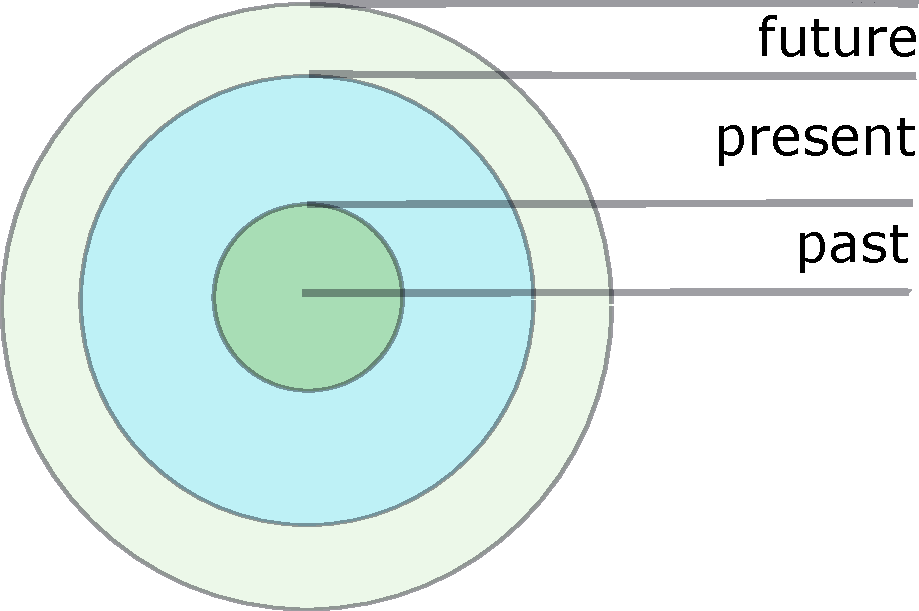
\includegraphics[height=100px]{node-glyph}
    \caption{The inner-most circle of the node glyph encodes the number of times
  the musician played in \emph{some} session in the past. The middle circle (blue)
  represents the number of sessions the musician played with the main musician
  within the current time frame. The radius of the outer largest circle encodes
  the total number of sessions the musician played throughout his/her career with
  or without the main musician.}
    \label{fig:node_glyphs}
  \end{figure}

  Node glyphs (Fig.~\ref{fig:node_glyphs}) consist of three concentric circles.
  The inner circle's radius is proportional to the square root of the count of
  sessions this musician played in the past, i.e. before the sessions currently
  visible on the timeline. The second circle's radius represents the square root
  of  the number of sessions from both the past and currently visible on the
  timeline in which that collaborator recorded. The radius of the outer circle is
  proportional to the square root of the total number of sessions the musician has
  recorded throughout their life. As users navigate the timeline in the direction
  of the future, more sessions would transfer to the ``past'' circle, increasing
  the radius of the inner-most circle. The radius of the circle representing the
  ``past+present'' may fluctuate depending on the number of sessions currently
  visible on the timeline. The radius of the outer circle, i.e. the square root of
  a total number of sessions recorded, does not change.

  Edge glyphs encode information about the overall count of recording sessions in
  which both the main musician and the collaborator participated
  (Fig.~\ref{fig:edge_glyphs} and~\ref{fig:duke-ell}). Edges are colored in varying shades of gray with
  the inner edge representing collaborations in the ``past'' and its thickness
  proportional to the square root of the number of sessions he or she shared with
  the main musician in the past. The thickness of the middle part is proportional
  to the root of the number of sessions for that collaborator currently visible on
  the timeline. Finally, the total edge thickness represents the number of
  sessions the two musicians played together overall.
   As users interact with the timeline, the thickness of the
  inner edges may change depending on the number of shared sessions in the past or
  currently visible on the timeline; however, the total thickness of an edge would
  not change.

  \begin{figure}[ht]
    \centering
    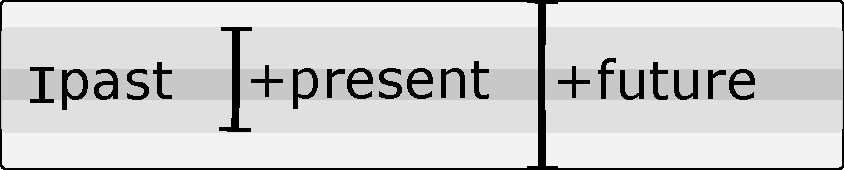
\includegraphics[width=0.7\linewidth]{edge-glyph}
    \caption{Edge glyph. The thickness of the inner-most inset in the edge glyph
  is proportional to the number of sessions the main musician and their
  collaborator played in the past, and the thickness of the "present" inset
  corresponds to the count of sessions in the past and present. The total edge
  thickness represents the number of sessions the two musicians played together
  overall.}
    \label{fig:edge_glyphs}
  \end{figure}

  Various combinations of node and edge thicknesses should alert the users to
  different modes of collaboration. A combination of a large peripheral node and a
  narrow edge connecting it to the center indicates that while the collaborator
  has played many sessions overall, they played very few with the main musician
  (for example, Don Redman in Fig.~\ref{fig:duke-ell}).
  Further, if the node's inner ``past'' circle is large, such combination then
  indicates that the collaborator is an established musician who is sharing their
  skills with the up and coming musician at the center of the ego-network. On the
  contrary, if the inner ``past'' circle is small and the majority of sessions are
  in the ``future'', such behavior may indicate that the collaborator has joined
  the main musician briefly and later went on to form an active career of their
  own. A case where both the node and the edge are thick indicates that the two
  musicians have recorded many sessions together and, therefore, share a strong
  tie.

  %%%%%%%%%%%%%%%%%%%%%%%%%%%%%%%%%%%%%%%%%%%%%%%%%%%%%%%%%%%%%%%%%%%%%%%%%%%%%%%%
  %
  % Visual: hops
  %
  %%%%%%%%%%%%%%%%%%%%%%%%%%%%%%%%%%%%%%%%%%%%%%%%%%%%%%%%%%%%%%%%%%%%%%%%%%%%%%%%

  \subsection{Exploring collaborators' connectivity}

  An ego-network allows users to focus on the dynamics of a few collaborations at
  the expense of hiding all other topological information. Knowing which, if any,
  peripheral nodes collaborate with each other helps to understand the communities
  that form in the immediate neighborhood of the main musician. The Map of Jazz
  provides such details on demand: when users hover over a collaborator's node $v$,
  the Map renders additional edges that connect $v$ to the collaborators it shares
  with the central node (Fig.~\ref{fig:young}). The thickness of the edges
  corresponds to the number of
  sessions the two musicians played in the past (including those they played
  with the main musician). When the edges connecting the main node and the
  performers on the periphery are thin indicating few collaborations, it would be
  noteworthy to see thick edges between those performers. Such a situation would
  imply that those artists form a strong community, or a band, outside of the main
  musician's neighborhood.

  %%%%%%%%%%%%%%%%%%%%%%%%%%%%%%%%%%%%%%%%%%%%%%%%%%%%%%%%%%%%%%%%%%%%%%%%%%%%%%%%
  %
  % User study
  %
  %%%%%%%%%%%%%%%%%%%%%%%%%%%%%%%%%%%%%%%%%%%%%%%%%%%%%%%%%%%%%%%%%%%%%%%%%%%%%%%%

  %\section{Evaluation}
\section{Usage Example with the Map of Jazz}

  \textbf{Duke Ellington}'s career spanned more than half a century from the
  early twenties to his death in 1974. The first record on the Map's timeline
  dates back to July of 1923 with Ellington playing piano and Elmer Snowden as the
  band leader --- Ellington was yet to form his own band. Ellington's egonet for
  the period of 1923--1928 has several prominent performer nodes: Harry Carney,
  Otto Hardwick, Sonny Greer, Fred Guy,  Barney Bigard, Joe Nanton, and Wellman
  Braud (see Fig.~\ref{fig:duke-ell}). The size of Harry Carney's node, for
  example, indicates that he participated in a significant number of recording
  sessions throughout his career (1487 sessions), and the thickness of the edge
  connecting him to Duke Ellington reveals that most of those sessions were
  recorded with Ellington (1480 sessions). The same holds for others in the list
  above: their careers were tightly knit with Ellington's.

  % overview of timeline

  From the details window, it is clear that Duke Ellington had a very productive
  career: over the course of his life he participated in more than 1740 sessions
  with 600 musicians. If the user zooms out on the timeline, it becomes evident
  how densely packed Ellington's recording sessions were, with the last
  right before his death. The pairwise session similarities that are visible on
  the timeline and the average pairwise similarity of 0.60 suggest that Ellington
  played with a core group of close collaborators who would replace one another
  over the years, but the band membership never changed all at once. Switching to
  the graph of session sizes, users can see that the average number of people per
  recording session was 14.19 (a size characteristic of big band ensembles) with
  the largest session at 29 performers recorded in January 1968.

  \begin{figure}[ht]
    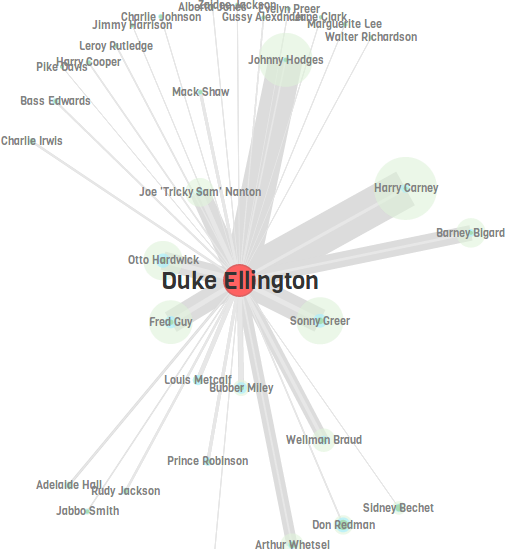
\includegraphics[width=\linewidth]{duke-ellington-1925-1928}
    \caption{Duke Ellington's ego-network during 1925--1928. His prominent
  collaborators can be easily identified by the thick edges.}
    \label{fig:duke-ell}
  \end{figure}

  % different bands

  Among Ellington's closest collaborators, several stopped collaborating with him
  either permanently or for a significant period of time. Ellington and Greer
  recorded 588 sessions together from 1923 to 1951, but there are no sessions
  past that: their collaboration ended after Greer's propensity for drinking
  forced Ellington to hire a second drummer to replace Greer. Apart from Greer,
  Johnny Hodges and Lawrence Brown, two of his most prominent collaborators, have
  a gap in recording sessions starting in 1951 which correlates with both
  musicians leaving the band to pursue their ambitions elsewhere. The recording
  sessions that included Hodges restart 5 years later and span all the way until
  his death in 1970; Brown rejoined the band later in 1960 to record 432 more
  sessions with Ellington.  The closely coupled timeline and ego-network displays
  allow such events to be found with relative ease.

  \textbf{Slide Hampton} has the most collaborators (1230) among all musicians
  represented in the Map of Jazz. He has composed and arranged music for many
  prominent musicians such as Kenny Barron, Chick Corea, Tommy Flanagan, Dizzy
  Gillespie, Clark Terry --- their large nodes stand out in Hampton's egonet ---
  as well as hundreds of lesser-known performers. Dragging the timeline across the
  length of his career shows that while at any given time period Hampton is
  connected to many artists, he rarely collaborated with them for prolonged
  periods of time: the collaborators' nodes do not move close to Hampton's central
  node, but rather stay at the periphery. The difference in collaboration style
  between Ellington and Hampton is especially pronounced when one compares their
  average sessions similarity (visible on the timeline): Hampton's average session
  similarity is at 0.19 compared to 0.60 for Duke Ellington. The average session
  size for Hampton is 12.09 --- combined with the low session similarity,
  we can conclude that Hampton accumulated the highest number of total
  collaborations by continuously seeking out new collaborators.

  \textbf{Count Basie}'s sessions account for 159 sessions available in the Map
  of Jazz, and his number of collaborators (253) seems modest when compared to
  Slide Hampton or Duke Ellington (see Fig.\@\ref{fig:map}). The first session
  available in the Map of Jazz dates back to 1936, when Basie acted as a band
  leader and pianist and \textbf{Lester Young} was on tenor sax (the roles of each musician
  in each session are available by mousing over the session in the timeline). The
  large size of Young's node in the ego-network foretells his successful
  career --- indeed, later he became one of the most influential saxophone
  players.

  By double-clicking on Young's node, we can start navigating through his
  personal timeline. Young recorded with Basie often in the 1930s and 1940s. The
  records are sparse for the period of 1941--1945: first due to an American
  Federation of Musicians' recording ban that stopped all commercial recording in
  1942--1944, then due to Young's being drafted into
  the army and serving a year-long jail term after being dishonorably discharged
  from service. Again, this gap in jazz productivity is clear from the display of
  sessions in the timeline.  Among his later collaborators are Billie Holiday,
  Charlie Parker, Buck Clayton, and Coleman Hawkins with whom Young recorded
  several times in 1946. The ``hops'' edges reveal that Parker, Clayton,
  and Hawkins had numerous sessions that did not include Young (see
  Fig.~\ref{fig:young}).

  \begin{figure}[ht]
    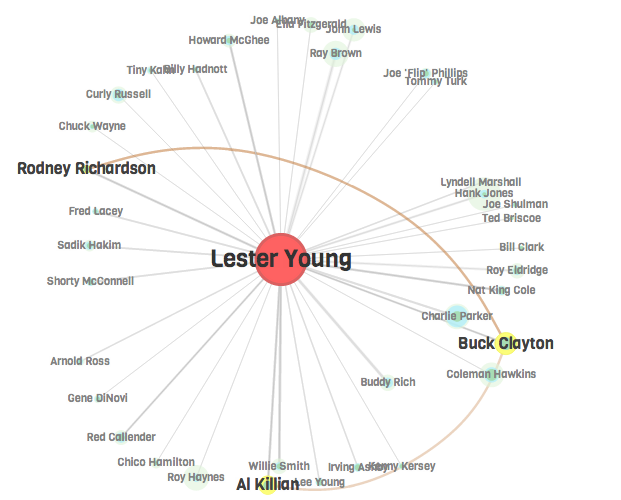
\includegraphics[width=\linewidth]{lester-young}
    \caption{Additional "hops" edges show past collaborations between periphery
  nodes that did not include the main musician. Here, Buck Clayton had recorded
  with Rodney Richardson and Al Killian numerous times prior to
  working with Lester Young.}
    \label{fig:young}
  \end{figure}

\section{Discussion and Conclusions}

  The Map of Jazz approaches the problem of dynamic graph visualization from a new
  angle: instead of tackling the hard problem of visualizing large graphs and
  tracking temporal changes on a global scale, the Map focuses on individual
  nodes and local changes that would have an immediate and personal effect. The Map
  of Jazz arranges related nodes into an ego-network with a single individual in
  the center surrounded by close neighbors who are placed according to the
  strength of their connection with the central node. Users can explore the
  dynamic properties of the network by dragging the time slider or zooming in on
  a particular era of interest. The ego-network adjusts the node positions
  according to the varying strength of their connection to the central node
  during that time. The appearance of nodes and edges updates as well to reflect
  the change in their attributes.

  We tailor our visualization to assist the exploration of a novel jazz
  collaboration network. In social interactions, the frequency and recency of
  interactions determine the strength of the collaboration between individuals.
  We propose and implement a collaboration strength function that takes into account both
  past and future interactions and helps quantify the strength of the
  relationship between the two musicians at any point in time.

  The concepts developed for the Map of Jazz can be applied to other social
  networks that record multiple interactions between individuals and to dynamic
  networks in general, especially those where the numerical attributes on nodes
  and edges change over time. One such example is the gene co-expression network
  where genes control the expression of other genes in the
  cell. The amount of one gene product may change over the natural cycle of a cell
  (cell division, growth, death) and affect the behavior of related genes.
  Applications to other collaboration networks such as co-authorship data are
  straightforward.



%%%%%%%%%%%%%%%%%%%%%%%%%%%%%%%%%%%%%%%%%%%%%%%%%%%%%%%%%%%%%%%%%%%%%%%%%%%%%%%%
%%
%% Map of jazz -- dynamic network vis
%%
%%%%%%%%%%%%%%%%%%%%%%%%%%%%%%%%%%%%%%%%%%%%%%%%%%%%%%%%%%%%%%%%%%%%%%%%%%%%%%%%
\chapter{Search interface for high-throughput sequencing metadata}

\section{Background}

SHARQ~\cite{SHARQwebsite}.

\section{Interface}

\section{Discussion and conclusions}


%%%%%%%%%%%%%%%%%%%%%%%%%%%%%%%%%%%%%%%%%%%%%%%%%%%%%%%%%%%%%%%%%%%%%%%%%%%%%%%%
%%
%% Coral --
%%
%%%%%%%%%%%%%%%%%%%%%%%%%%%%%%%%%%%%%%%%%%%%%%%%%%%%%%%%%%%%%%%%%%%%%%%%%%%%%%%%
\chapter{Interfaces for evaluation and comparison of classification results}

This work appears as a stand-alone publication in BMC Bioinformatics~\cite{Filippova2012}.

\section{Background and related work}

  (abstract)

  Clustering has become a standard analysis  for many
  types of biological data (\eg~interaction networks, gene expression,
  metagenomic abundance). In practice, it is possible to obtain a large number of
  contradictory clusterings by varying which clustering algorithm is used, which
  data attributes are considered, how algorithmic parameters are set, and  which
  near-optimal clusterings are chosen. It is a difficult task to sift though such
  a large collection of varied clusterings to determine which clustering features
  are affected by parameter settings or are artifacts of particular algorithms and
  which represent meaningful patterns. Knowing which items are often clustered
  together helps to improve our understanding of the underlying data and to
  increase our confidence about generated modules.

  \paragraph{Results} We present \Coral, an application for interactive
  exploration of large ensembles of clusterings. \Coral makes all-to-all
  clustering comparison easy, supports exploration of individual clusterings,
  allows tracking modules across clusterings, and supports identification of core
  and peripheral items in modules. We discuss how each visual component in \Coral
  tackles a specific question related to clustering comparison and provide
  examples of their use. We also show how \Coral could be used to visually and
  quantitatively compare clusterings with a ground truth clustering.

  \paragraph{Conclusion} As a case study, we compare clusterings of a recently
  published protein interaction network of \textit{Arabidopsis thaliana}. We use
  several popular algorithms to generate the network's clusterings. We find that
  the clusterings vary significantly and that few proteins are consistently
  co-clustered in all clusterings. This is evidence that several clusterings
  should typically be considered when evaluating modules of genes, proteins, or
  sequences, and Coral can be used to perform a comprehensive analysis of these
  clustering ensembles.

  (introduction)

  Collections of protein interactions, gene expression vectors, metagenomic
  samples, and gene sequences containing thousands to hundreds-of-thousands of
  elements are now being analyzed routinely. Clustering is often used to condense
  such large datasets into an understandable form: it has been successfully used
  on protein-protein interaction (PPI) networks to discover protein complexes and
  predict protein function, \eg~\cite{Sharan2007}; on gene expression data to find
  patterns in gene regulation and essential cell processes, \eg~\cite{Ulitsky2010};
  and on metagenomic samples to identify new species, compare them to existing
  clades, evaluate the diversity of a population, and suggest interdependencies
  between them~\cite{Chatterji2007, White2010}. In other words, clustering has
  become a ubiquitous part of analysis for large biological datasets.

  % Introduce the problem.

  There are many clustering algorithms available for numerical and network data,
  \eg~\cite{VanDongen2000, Bader2003, Clauset2004, Adamcsek2006, Blondel2008,
  Ahn2010, Jiang2010, Rhrissorrakrai2011}. Each algorithm, and choice of its
  parameters, results in different clusterings.
  Sometimes, clustering algorithms must resolve ties when generating modules or
  may be randomized. Consequently, a single clustering algorithm may produce
  diverse partitions on the same data~\cite{Navlakha10}. Clusterings may also
  change when the underlying data becomes increasingly noisy or displays
  variation under different conditions (such as varying gene expression levels).
  In addition, considering many optimal and
  near-optimal partitions has been shown to improve the understanding of module
  dynamics and the strength of relationships between individual
  items~\cite{Duggal2010, Lewis2010, Langfelder2008, Hopcroft2004}. Such
  clusterings may offer drastically different perspectives on the data, where
  assessing the commonalities and differences is of great interest.

  % existing solutions

  There are several ways in which the problem of diverse clusterings has been
  addressed. Some tools rely on a single clustering only and focus on module
  quality assessment, \eg~\cite{Yu2007a, Hibbs2005}. Comparing two or more
  clusterings at a time is usually done by computing a single metric, such as the
  Jaccard or Rand index~\cite{Thalamuthu2006}, to compare clusterings
  side-by-side~\cite{Seo2007a} or in a dendrogram~\cite{Laderas2007}. These
  approaches can easily compare a pair of clusterings, but are not extendable to
  greater number of clusterings. Another approach is to aggregate multiple
  partitions into a consensus clustering~\cite{strehl02, Monti2003a} without
  delving into the differences between individual clusterings and, thus,
  disregarding possibly important information about the clusterings. Finally, some
  approaches have made steps towards visual examination of multiple clusterings:
  King and Grimmer~\cite{Grimmer2011} compare clusterings pairwise and project the
  space of clusterings onto a plane to visualize a clustering landscape, and
  Langfelder et al.~\cite{Langfelder2011} investigate ways to compare individual
  modules across multiple conditions.{{\pagebreak}\break} However, none of these approaches offer a
  platform for a multi-level analysis of ensembles of diverse clusterings.

\section{Interface design}

  In \Coral's design, we followed the visualization mantra coined by
  Shneiderman~\cite{Shneiderman1996}: overview, zoom-and-filter,
  details-on-demand. At the overview level, \Coral displays dataset statistics and
  highlights the most similar and dissimilar clusterings; at the mid-level,
  ``zoomed-in,'' analysis explains similarities between clusterings through module
  comparison; the low-level analysis compares co-clustering patterns at the level
  of individual data items: the genes, proteins, or sequences. The displays are
  coordinated~\cite{North2000} so selecting data in one of the views highlights
  the corresponding items in the other views (see Figure 1).

  %== Figure 1 ==
  \hrulefill \\
  \textbf{Figure 1 Coral overview.}
  Coral views in a clockwise direction: co-cluster matrix (1), pairs table (2),
  parallel partitions plot (3), module-to-module table (4), ladder (5), overview
  statistics (6). Users may rearrange the individual views or close them to focus
  on fewer visualizations at a time. Data: \Athal clusterings.
  \\[-6pt]\hrulefill \\

  \vspace*{12pt}
  Coral works with modules --- groups of items closely related to one
  another according to some metric or property. For example, modules can
  constitute a collection of genes that get co-expressed together or proteins
  forming a complex. A clustering is a collection of modules and usually is an
  output of a clustering algorithm. Users may also choose to group data according
  to attributes that come with the data such as cellular component or molecular
  function GO terms and use that partition as a clustering. Users may combine data
  from different experiemnts and across species so long as the data items that the
  user treats as homologous have the same IDs across the dataset.

  \Coral takes as an input the module files where each file represents a single
  clustering, and each line in the file contains a list of data items (proteins,
  genes, or sequence ids) from a single module, \eg~as produced by MCL,
  the clustering algorithm by van Dongen~\cite{VanDongen2000}. \Coral aggregates
  and visualizes these data through several connected displays, each of which can
  be used to answer specific questions about the clusterings. Below, we examine a
  few such questions and describe how \Coral's visualizations help to answer them.

  

\section{Results and discussion}

\section{Conclusions}


%%%%%%%%%%%%%%%%%%%%%%%%%%%%%%%%%%%%%%%%%%%%%%%%%%%%%%%%%%%%%%%%%%%%%%%%%%%%%%%%
%%%%%%%%%%%%%%%%%%%%%%%%%%%%%%%%%%%%%%%%%%%%%%%%%%%%%%%%%%%%%%%%%%%%%%%%%%%%%%%%
%%
%%
%%
%% Part 2 -- high-level structure and compression
%%
%%
%%
%%%%%%%%%%%%%%%%%%%%%%%%%%%%%%%%%%%%%%%%%%%%%%%%%%%%%%%%%%%%%%%%%%%%%%%%%%%%%%%%
%%%%%%%%%%%%%%%%%%%%%%%%%%%%%%%%%%%%%%%%%%%%%%%%%%%%%%%%%%%%%%%%%%%%%%%%%%%%%%%%
\part{Inferring structure and its use in data compression}

%%%%%%%%%%%%%%%%%%%%%%%%%%%%%%%%%%%%%%%%%%%%%%%%%%%%%%%%%%%%%%%%%%%%%%%%%%%%%%%%
%%
%% Domains -- inferring high-level structure from DNA conformation data
%%
%%%%%%%%%%%%%%%%%%%%%%%%%%%%%%%%%%%%%%%%%%%%%%%%%%%%%%%%%%%%%%%%%%%%%%%%%%%%%%%%
% algorithms for managing biological data
\chapter{Identifying high-level structure in DNA conformation data}

\section{Background and related work}

Domains, cha!~\cite{Filippova2013}, hierarchical domains~\cite{ArmatusAMB}.

\section{Results and discussion}

\section{Conclusions}


%%%%%%%%%%%%%%%%%%%%%%%%%%%%%%%%%%%%%%%%%%%%%%%%%%%%%%%%%%%%%%%%%%%%%%%%%%%%%%%%
%%
%% Huffmer and Referee -- compression projects
%%
%%%%%%%%%%%%%%%%%%%%%%%%%%%%%%%%%%%%%%%%%%%%%%%%%%%%%%%%%%%%%%%%%%%%%%%%%%%%%%%%
\chapter{Compression of sequencing data and alignment information}

\section{Background}

\section{De novo sequence compression}

\section{Reference-based sequence compression}

\section{Results and discussion}

\section{Conclusions}

Referee~\cite{Referee_draft}


%%%%%%%%%%%%%%%%%%%%%%%%%%%%%%%%%%%%%%%%%%%%%%%%%%%%%%%%%%%%%%%%%%%%%%%%%%%%%%%%
%%
%% Overall conclusions
%%
%%%%%%%%%%%%%%%%%%%%%%%%%%%%%%%%%%%%%%%%%%%%%%%%%%%%%%%%%%%%%%%%%%%%%%%%%%%%%%%%
\chapter{Discussion and Conclusions}

XXX

%\appendix
%\include{appendix}

\backmatter

%\renewcommand{\baselinestretch}{1.0}\normalsize

% By default \bibsection is \chapter*, but we really want this to show
% up in the table of contents and pdf bookmarks.
\renewcommand{\bibsection}{\chapter{\bibname}}
%\newcommand{\bibpreamble}{This text goes between the ``Bibliography''
%  header and the actual list of references}
\bibliographystyle{plainnat}
\bibliography{mypapers,references,jazzmap,graph_drawing,dynnetvis} %your bib file

\end{document}
